%% bare_conf_compsoc.tex
%% V1.4b
%% 2015/08/26
%% by Michael Shell
%% See:
%% http://www.michaelshell.org/
%% for current contact information.
%%
%% This is a skeleton file demonstrating the use of IEEEtran.cls
%% (requires IEEEtran.cls version 1.8b or later) with an IEEE Computer
%% Society conference paper.
%%
%% Support sites:
%% http://www.michaelshell.org/tex/ieeetran/
%% http://www.ctan.org/pkg/ieeetran
%% and
%% http://www.ieee.org/

%%*************************************************************************
%% Legal Notice:
%% This code is offered as-is without any warranty either expressed or
%% implied; without even the implied warranty of MERCHANTABILITY or
%% FITNESS FOR A PARTICULAR PURPOSE! 
%% User assumes all risk.
%% In no event shall the IEEE or any contributor to this code be liable for
%% any damages or losses, including, but not limited to, incidental,
%% consequential, or any other damages, resulting from the use or misuse
%% of any information contained here.
%%
%% All comments are the opinions of their respective authors and are not
%% necessarily endorsed by the IEEE.
%%
%% This work is distributed under the LaTeX Project Public License (LPPL)
%% ( http://www.latex-project.org/ ) version 1.3, and may be freely used,
%% distributed and modified. A copy of the LPPL, version 1.3, is included
%% in the base LaTeX documentation of all distributions of LaTeX released
%% 2003/12/01 or later.
%% Retain all contribution notices and credits.
%% ** Modified files should be clearly indicated as such, including  **
%% ** renaming them and changing author support contact information. **
%%*************************************************************************


% *** Authors should verify (and, if needed, correct) their LaTeX system  ***
% *** with the testflow diagnostic prior to trusting their LaTeX platform ***
% *** with production work. The IEEE's font choices and paper sizes can   ***
% *** trigger bugs that do not appear when using other class files.       ***                          ***
% The testflow support page is at:
% http://www.michaelshell.org/tex/testflow/



\documentclass[conference,compsoc]{IEEEtran}
% Some/most Computer Society conferences require the compsoc mode option,
% but others may want the standard conference format.
%
% If IEEEtran.cls has not been installed into the LaTeX system files,
% manually specify the path to it like:
% \documentclass[conference,compsoc]{../sty/IEEEtran}





% Some very useful LaTeX packages include:
% (uncomment the ones you want to load)


% *** MISC UTILITY PACKAGES ***
%
%\usepackage{ifpdf}
% Heiko Oberdiek's ifpdf.sty is very useful if you need conditional
% compilation based on whether the output is pdf or dvi.
% usage:
% \ifpdf
%   % pdf code
% \else
%   % dvi code
% \fi
% The latest version of ifpdf.sty can be obtained from:
% http://www.ctan.org/pkg/ifpdf
% Also, note that IEEEtran.cls V1.7 and later provides a builtin
% \ifCLASSINFOpdf conditional that works the same way.
% When switching from latex to pdflatex and vice-versa, the compiler may
% have to be run twice to clear warning/error messages.






% *** CITATION PACKAGES ***
%
\ifCLASSOPTIONcompsoc
  % IEEE Computer Society needs nocompress option
  % requires cite.sty v4.0 or later (November 2003)
  \usepackage[nocompress]{cite}
\else
  % normal IEEE
  \usepackage{cite}
\fi
% cite.sty was written by Donald Arseneau
% V1.6 and later of IEEEtran pre-defines the format of the cite.sty package
% \cite{} output to follow that of the IEEE. Loading the cite package will
% result in citation numbers being automatically sorted and properly
% "compressed/ranged". e.g., [1], [9], [2], [7], [5], [6] without using
% cite.sty will become [1], [2], [5]--[7], [9] using cite.sty. cite.sty's
% \cite will automatically add leading space, if needed. Use cite.sty's
% noadjust option (cite.sty V3.8 and later) if you want to turn this off
% such as if a citation ever needs to be enclosed in parenthesis.
% cite.sty is already installed on most LaTeX systems. Be sure and use
% version 5.0 (2009-03-20) and later if using hyperref.sty.
% The latest version can be obtained at:
% http://www.ctan.org/pkg/cite
% The documentation is contained in the cite.sty file itself.
%
% Note that some packages require special options to format as the Computer
% Society requires. In particular, Computer Society  papers do not use
% compressed citation ranges as is done in typical IEEE papers
% (e.g., [1]-[4]). Instead, they list every citation separately in order
% (e.g., [1], [2], [3], [4]). To get the latter we need to load the cite
% package with the nocompress option which is supported by cite.sty v4.0
% and later.





% *** GRAPHICS RELATED PACKAGES ***
%
\ifCLASSINFOpdf
  \usepackage[pdftex]{graphicx}
  % declare the path(s) where your graphic files are
  \graphicspath{{../pdf/}{../jpeg/}{./figures/}}
  % and their extensions so you won't have to specify these with
  % every instance of \includegraphics
  \DeclareGraphicsExtensions{.pdf,.jpeg,.png}
\else
  % or other class option (dvipsone, dvipdf, if not using dvips). graphicx
  % will default to the driver specified in the system graphics.cfg if no
  % driver is specified.
  % \usepackage[dvips]{graphicx}
  % declare the path(s) where your graphic files are
  % \graphicspath{{../eps/}}
  % and their extensions so you won't have to specify these with
  % every instance of \includegraphics
  % \DeclareGraphicsExtensions{.eps}
\fi
% graphicx was written by David Carlisle and Sebastian Rahtz. It is
% required if you want graphics, photos, etc. graphicx.sty is already
% installed on most LaTeX systems. The latest version and documentation
% can be obtained at: 
% http://www.ctan.org/pkg/graphicx
% Another good source of documentation is "Using Imported Graphics in
% LaTeX2e" by Keith Reckdahl which can be found at:
% http://www.ctan.org/pkg/epslatex
%
% latex, and pdflatex in dvi mode, support graphics in encapsulated
% postscript (.eps) format. pdflatex in pdf mode supports graphics
% in .pdf, .jpeg, .png and .mps (metapost) formats. Users should ensure
% that all non-photo figures use a vector format (.eps, .pdf, .mps) and
% not a bitmapped formats (.jpeg, .png). The IEEE frowns on bitmapped formats
% which can result in "jaggedy"/blurry rendering of lines and letters as
% well as large increases in file sizes.
%
% You can find documentation about the pdfTeX application at:
% http://www.tug.org/applications/pdftex





% *** MATH PACKAGES ***
%
%\usepackage{amsmath}
% A popular package from the American Mathematical Society that provides
% many useful and powerful commands for dealing with mathematics.
%
% Note that the amsmath package sets \interdisplaylinepenalty to 10000
% thus preventing page breaks from occurring within multiline equations. Use:
%\interdisplaylinepenalty=2500
% after loading amsmath to restore such page breaks as IEEEtran.cls normally
% does. amsmath.sty is already installed on most LaTeX systems. The latest
% version and documentation can be obtained at:
% http://www.ctan.org/pkg/amsmath





% *** SPECIALIZED LIST PACKAGES ***
%
%\usepackage{algorithmic}
% algorithmic.sty was written by Peter Williams and Rogerio Brito.
% This package provides an algorithmic environment fo describing algorithms.
% You can use the algorithmic environment in-text or within a figure
% environment to provide for a floating algorithm. Do NOT use the algorithm
% floating environment provided by algorithm.sty (by the same authors) or
% algorithm2e.sty (by Christophe Fiorio) as the IEEE does not use dedicated
% algorithm float types and packages that provide these will not provide
% correct IEEE style captions. The latest version and documentation of
% algorithmic.sty can be obtained at:
% http://www.ctan.org/pkg/algorithms
% Also of interest may be the (relatively newer and more customizable)
% algorithmicx.sty package by Szasz Janos:
% http://www.ctan.org/pkg/algorithmicx




% *** ALIGNMENT PACKAGES ***
%
%\usepackage{array}
% Frank Mittelbach's and David Carlisle's array.sty patches and improves
% the standard LaTeX2e array and tabular environments to provide better
% appearance and additional user controls. As the default LaTeX2e table
% generation code is lacking to the point of almost being broken with
% respect to the quality of the end results, all users are strongly
% advised to use an enhanced (at the very least that provided by array.sty)
% set of table tools. array.sty is already installed on most systems. The
% latest version and documentation can be obtained at:
% http://www.ctan.org/pkg/array


% IEEEtran contains the IEEEeqnarray family of commands that can be used to
% generate multiline equations as well as matrices, tables, etc., of high
% quality.




% *** SUBFIGURE PACKAGES ***
%\ifCLASSOPTIONcompsoc
%  \usepackage[caption=false,font=footnotesize,labelfont=sf,textfont=sf]{subfig}
%\else
%  \usepackage[caption=false,font=footnotesize]{subfig}
%\fi
% subfig.sty, written by Steven Douglas Cochran, is the modern replacement
% for subfigure.sty, the latter of which is no longer maintained and is
% incompatible with some LaTeX packages including fixltx2e. However,
% subfig.sty requires and automatically loads Axel Sommerfeldt's caption.sty
% which will override IEEEtran.cls' handling of captions and this will result
% in non-IEEE style figure/table captions. To prevent this problem, be sure
% and invoke subfig.sty's "caption=false" package option (available since
% subfig.sty version 1.3, 2005/06/28) as this is will preserve IEEEtran.cls
% handling of captions.
% Note that the Computer Society format requires a sans serif font rather
% than the serif font used in traditional IEEE formatting and thus the need
% to invoke different subfig.sty package options depending on whether
% compsoc mode has been enabled.
%
% The latest version and documentation of subfig.sty can be obtained at:
% http://www.ctan.org/pkg/subfig




% *** FLOAT PACKAGES ***
%
%\usepackage{fixltx2e}
% fixltx2e, the successor to the earlier fix2col.sty, was written by
% Frank Mittelbach and David Carlisle. This package corrects a few problems
% in the LaTeX2e kernel, the most notable of which is that in current
% LaTeX2e releases, the ordering of single and double column floats is not
% guaranteed to be preserved. Thus, an unpatched LaTeX2e can allow a
% single column figure to be placed prior to an earlier double column
% figure.
% Be aware that LaTeX2e kernels dated 2015 and later have fixltx2e.sty's
% corrections already built into the system in which case a warning will
% be issued if an attempt is made to load fixltx2e.sty as it is no longer
% needed.
% The latest version and documentation can be found at:
% http://www.ctan.org/pkg/fixltx2e


%\usepackage{stfloats}
% stfloats.sty was written by Sigitas Tolusis. This package gives LaTeX2e
% the ability to do double column floats at the bottom of the page as well
% as the top. (e.g., "\begin{figure*}[!b]" is not normally possible in
% LaTeX2e). It also provides a command:
%\fnbelowfloat
% to enable the placement of footnotes below bottom floats (the standard
% LaTeX2e kernel puts them above bottom floats). This is an invasive package
% which rewrites many portions of the LaTeX2e float routines. It may not work
% with other packages that modify the LaTeX2e float routines. The latest
% version and documentation can be obtained at:
% http://www.ctan.org/pkg/stfloats
% Do not use the stfloats baselinefloat ability as the IEEE does not allow
% \baselineskip to stretch. Authors submitting work to the IEEE should note
% that the IEEE rarely uses double column equations and that authors should try
% to avoid such use. Do not be tempted to use the cuted.sty or midfloat.sty
% packages (also by Sigitas Tolusis) as the IEEE does not format its papers in
% such ways.
% Do not attempt to use stfloats with fixltx2e as they are incompatible.
% Instead, use Morten Hogholm'a dblfloatfix which combines the features
% of both fixltx2e and stfloats:
%
% \usepackage{dblfloatfix}
% The latest version can be found at:
% http://www.ctan.org/pkg/dblfloatfix




% *** PDF, URL AND HYPERLINK PACKAGES ***
%
\usepackage{url}
% url.sty was written by Donald Arseneau. It provides better support for
% handling and breaking URLs. url.sty is already installed on most LaTeX
% systems. The latest version and documentation can be obtained at:
% http://www.ctan.org/pkg/url
% Basically, \url{my_url_here}.


\usepackage{units}
%\usepackage{nicefrac}

\usepackage{etoolbox}
\newtoggle{inclIEEECopyRight}
\toggletrue{inclIEEECopyRight}


% *** Do not adjust lengths that control margins, column widths, etc. ***
% *** Do not use packages that alter fonts (such as pslatex).         ***
% There should be no need to do such things with IEEEtran.cls V1.6 and later.
% (Unless specifically asked to do so by the journal or conference you plan
% to submit to, of course. )


% correct bad hyphenation here
\hyphenation{op-tical net-works semi-conduc-tor}


\begin{document}
\iftoggle{inclIEEECopyRight}{
    \begin{titlepage}
    \mbox{}\\{\Large \textbf{IEEE Copyright Notice}}
    \newline\newline\newline\newline
    \textcopyright~2021 IEEE. Personal use of this material is permitted.
    Permission from IEEE must be obtained for all other uses, in any current
    or future media, including reprinting/republishing this material for
    advertising or promotional purposes, creating new collective works, for
    resale or redistribution to servers or lists, or reuse of any copyrighted
    component of this work in other works.
    \newline\newline\newline\newline
    {\large Accepted to be Published in: Proceedings of the 2021 {IEEE}
    {International} {Conference} on {Cluster} {Computing} ({CLUSTER}), {EAHPC}
    {Workshop}, Sept. 7-10, 2021 Portland, Oregon, USA}
    \end{titlepage}
}{}

\bstctlcite{IEEEexample:BSTcontrol}
%\linenumbers
%\linenumbersep 3pt\relax

%
% paper title
% Titles are generally capitalized except for words such as a, an, and, as,
% at, but, by, for, in, nor, of, on, or, the, to and up, which are usually
% not capitalized unless they are the first or last word of the title.
% Linebreaks \\ can be used within to get better formatting as desired.
% Do not put math or special symbols in the title.
\title{A64FX -- Your Compiler You Must Decide!}


% author names and affiliations
% use a multiple column layout for up to three different
% affiliations
\author{\IEEEauthorblockN{Jens Domke}
\IEEEauthorblockA{RIKEN Center for Computational Science (R-CCS)\\
Kobe, Hyogo, 650-0047 Japan\\
Email: \url{http://domke.gitlab.io/##contact}}}

% conference papers do not typically use \thanks and this command
% is locked out in conference mode. If really needed, such as for
% the acknowledgment of grants, issue a \IEEEoverridecommandlockouts
% after \documentclass

% for over three affiliations, or if they all won't fit within the width
% of the page (and note that there is less available width in this regard for
% compsoc conferences compared to traditional conferences), use this
% alternative format:
% 
%\author{\IEEEauthorblockN{Michael Shell\IEEEauthorrefmark{1},
%Homer Simpson\IEEEauthorrefmark{2},
%James Kirk\IEEEauthorrefmark{3}, 
%Montgomery Scott\IEEEauthorrefmark{3} and
%Eldon Tyrell\IEEEauthorrefmark{4}}
%\IEEEauthorblockA{\IEEEauthorrefmark{1}School of Electrical and Computer Engineering\\
%Georgia Institute of Technology,
%Atlanta, Georgia 30332--0250\\ Email: see http://www.michaelshell.org/contact.html}
%\IEEEauthorblockA{\IEEEauthorrefmark{2}Twentieth Century Fox, Springfield, USA\\
%Email: homer@thesimpsons.com}
%\IEEEauthorblockA{\IEEEauthorrefmark{3}Starfleet Academy, San Francisco, California 96678-2391\\
%Telephone: (800) 555--1212, Fax: (888) 555--1212}
%\IEEEauthorblockA{\IEEEauthorrefmark{4}Tyrell Inc., 123 Replicant Street, Los Angeles, California 90210--4321}}




% use for special paper notices
%\IEEEspecialpapernotice{(Invited Paper)}




% make the title area
\maketitle

% As a general rule, do not put math, special symbols or citations
% in the abstract
\begin{abstract}
The current number one of the TOP500 list, Supercomputer Fugaku, has demonstrated that CPU-only HPC
systems aren't dead and CPUs can be used for more than just being the host controller for a discrete accelerators.
While the specifications of the chip and overall system architecture, and benchmarks submitted to
various lists, like TOP500 and Green500, etc., are clearly highlighting the potential, the proliferation
of Arm into the HPC business is rather recent and hence the software stack might not be fully matured
and tuned, yet. We test 3 state-of-the-art compiler suite against a broad set of benchmarks.
Our measurements show that orders of magnitudes in performance can be gained by deviating from the
recommended usage model of the A64FX compute nodes.
\end{abstract}

% no keywords




% For peer review papers, you can put extra information on the cover
% page as needed:
% \ifCLASSOPTIONpeerreview
% \begin{center} \bfseries EDICS Category: 3-BBND \end{center}
% \fi
%
% For peerreview papers, this IEEEtran command inserts a page break and
% creates the second title. It will be ignored for other modes.
\IEEEpeerreviewmaketitle



\section{Introduction}\label{sec:intro}
The HPC community has been testing Arm-based architectures for a few years
now~\cite{rajovic_supercomputing_2013,rajovic_mont-blanc_2016,rico_arm_2017}, and
Supercomputer Fugaku~\cite{sato_co-design_2020} is the first large-scale system in the top-end of the TOP500 list, which demonstrates the competitiveness
of Arm in
a space which recently had been dominated by Intel, AMD, and Nvidia. The benefits of Arm CPUs paired
with high bandwidth memory, as in the case of Fujitsu's A64FX processor~\cite{fujitsu_limited_fujitsu_nodate}, for the HPC field are clear:
(1) Arm CPUs are highly customizable, energy efficient, and there is an existing ecosystem of software,
compilers, tools, etc., which is readily available (unlike for the K computer with its SPARC CPU); and (2) most applications executed on HPC systems
tend to be memory-bandwidth-bound, as we have shown in a previous study~\cite{domke_double-precision_2019}.
Although, a different compute-to-bandwidth
ratio, as found in A64FX, might challenge this view in individual cases resulting in a greater influence
by the compiler onto the performance. Furthermore, despite the dominance of Arm chips in the embedded
and low-power space, the system software and compilers, such as the widely used GNU Compiler Collection
for embedded systems, might be tuned for metrics other than wide vectors (e.g., Arm's Scalable Vector
Extension) and high performance.

It is known among benchmarkers and performance analysts, that Intel’s Parallel Studio or AMD's AOCC compilers,
depending on the CPU vendor, usually yield a high baseline performance. However, for Fujitsu's A64FX, this
choice is not that obvious, yet, and options such as Fujitsu's compiler suite, GNU Compiler Collection,
Arm compilers, and HPE/Cray compilers exist, and need to be evaluated.

For example, after Supercomputer Fugaku---or short Fugaku hereafter---was put into production, we
experimented with micro kernels, namely PolyBench~\cite{pouchet_polybenchc_2016}, to debug some unexpected performance
discrepancies, especially when compared to an Intel Xeon E5-2650v4 reference CPU. While a compiler-based core-to-core
comparison for these single-threaded benchmarks is inherently inaccurate (due to ISA, caches, GHz, etc.), we did not expect
the Xeon to execute some tests up to two orders of magnitude faster, see Figure~\ref{fig:demo_polly}.
This obviously does not make sense, especially when looking at the \textit{2mm} and \textit{3mm}
matrix multiplication cases which should be compute-bound.
%
\begin{figure}[tbp]
    \centering
    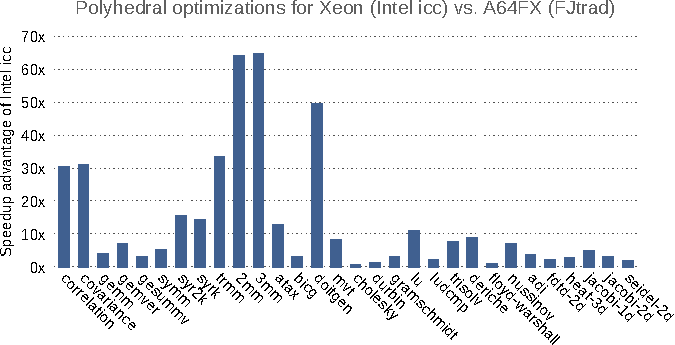
\includegraphics[width=0.96\linewidth]{demo_polly}
    \caption{\textbf{Unexpected advantage of Xeon vs.~A64FX} in PolyBench[large], which \textbf{prompted this study}.
    Recommended compiler/flags used for both.}
    \label{fig:demo_polly}
\end{figure}
%
We will analyze the reasons in greater depth in Section~\ref{sec:eval:micro}, and it initiated
this study in which we seek to answer the following questions:
\begin{itemize}
	\item Is the recommended usage model for A64FX, i.e., compiler+flags as well as number of MPI/OMP ranks
	and threads, ideal or just a starting point?
	\item Is there a ``silver bullet'' compiler choice for A64FX?
	\item Can performance differences, compared to similar x86-based hardware, be attributed to the compiler?
\end{itemize}
To answer these questions, our contributions are as follows:
\begin{itemize}
	\item We execute a broad set of micro benchmarks, procurement proxy applications, and real-world
	application benchmarks under 5 different compiler environments to determine performance trends.
	\item A detailed discussion of the performance opportunities arising from different compiler options
	(which can also create challenges for ordinary users), and recommendations for operators and users of A64FX.
\end{itemize}


\section{Measurement Methodology}\label{sec:metho}
The performance discrepancy for the \textit{2mm} benchmark was quickly identified. Intel's C compiler
reordered the nested loop construct, while Fujitsu's C compiler (fcc) failed to do so, resulting in a
64x speedup on the Xeon core which has less than \textonehalf~of a A64FX cores's theoretical peak flop/s.
Hence, we started investigating alternative compilers to improve PolyBench and also real-world codes on Fugaku.

\subsection{Compiler and Compiler Flags}\label{sec:metho:compiler}
\textbf{FUJITSU Software Technical Computing Suite (v4.5.0)} is the recommended compiler infrastructure
for Fugaku supporting C/C++ and Fortran. It supports two modes, \textit{traditional} and \textit{clang};
the latter being based on an enhanced version of LLVM 7. We utilize both modes in this study, and link
to Fujitsu's SSL2 library for linear algebra operations whenever necessary. Most application come with
build scripts tuned for individual compilers, and we augment them with \textit{-Kfast,ocl,largepage,lto}
for performance, optimization control line (OCL) support, hugepages, and link-time-optimization, respectively.

\textbf{LLVM Compiler Infrastructure (v12)} supports C/C++ via clang; however, flang (LLVM's Fortran frontend) requires
currently a host compiler and we experienced many errors using it, and hence we skip flang and directly utilize Fujitsu's \textit{frt} compiler.
We test two settings with LLVM, the first being \textit{-Ofast -ffast-math -flto=thin} and the second
specifically targeting polyhedral optimizations with \textit{-mllvm -polly -mllvm -polly-vectorizer=polly}
and replacing the thin linker with the full linker, since \textit{thin} interfered with \textit{polly}.

\textbf{GNU Compiler Collection (v10.2.0)} supports C/C++ and Fortran, and we use
\textit{-O3 -march=native -flto} in addition to the benchmark-specific compiler flags whenever possible.

Hence, we have 5 variations, identified hereafter with \textit{FJtrad}, \textit{FJclang}, \textit{LLVM},
\textit{LLVM+Polly}, and \textit{GNU}. Unless otherwise stated, the flags listed above (or minor
variations to avoid compile/runtime issues) are in effect\footnote{Compilation scripts \&  
inputs available: \url{gitlab.com/domke/a64fxCvC}}.

Other commercial compilers from Arm (a fork of LLVM with additional optimizations and native Fortran-support)
and HPE/Cray exist; however, these are currently not available on Fugaku and we could not install
them ourselves without acquiring a license. We refer an interested reader to our related work in Section~\ref{sec:relwork}
which includes comparison for these compilers as well, but on other benchmarks/systems.


\subsection{Benchmarks -- From Micro to Macro Level}\label{sec:metho:benchmarks}
We test over 100 different kernels and scientific codes from 7 benchmark suites, as outlined hereafter:

\textbf{Micro Kernels} are a collection of 22 kernels\footnote{Source code: \url{github.com/RIKEN-RCCS/fs2020-tapp-kernels};
We use earlier snapshot; Referencing them with Kernel 1$\ldots$22 to avoid confusion.} extracted from RIKEN priority applications (see
later in this Section), which have been used during the Fugaku development for testing and validation.
These kernels are OpenMP-parallelized, primarily written in Fortran (except 5), and test various
performance-relevant aspects of one core memory group (CMG) of the A64FX processor, i.e., 12 cores (+1 assistant/OS core)
and a \unit[8]{GiB} HBM2 module.

\textbf{Polyhedral Benchmark suite} (in short, PolyBench) is a collection of 30 single-threaded
scientific kernels written in C. The input sizes can be tuned for different memory hierarchy levels,
and we use the \textit{LARGE} input (exc.: \textit{MEDIUM} for \textit{floyd-warshall}) to stress all
memory levels of A64FX.

\textbf{HPL, HPCG, and BabelStream} are commonly known to test the system's compute~\cite{dongarra_linpack_1988} and
memory performance~\cite{dongarra_hpcg_2015,deakin_gpu-stream_2016}, and are used, for example, to rank supercomputers in the TOP500 list.
HPL's and HPCG's problem sizes are configured to 36,864 and 120\textsuperscript{3}, respectively, while we
use \unit[2]{GiByte} long vectors for the stream benchmark.

\textbf{ECP proxy-apps and RIKEN Fiber mini-apps} are collections of so called \textit{proxy applications}
which are smaller representative codes and inputs for production applications commonly executed on
supercomputers in the USA and Japan. We have studied these codes previously~\cite{domke_double-precision_2019,domke_matrix_2021},
and we refer the reader to these publications for details.

\textbf{SPEC CPU[speed] and OMP} are two suites used by HPC centers and vendors to test
compute node capabilities. The former comprises 20 tests. One half are single-threaded,
integer-intensive computations and the other half tests multi-threaded, floating-point-heavy scientific
applications. The latter are 14 science workloads which are OpenMP-parallelized, too. The benchmarks
are implemented in C, Fortran, and C++, or a mix thereof. For our (non-compliant) SPEC runs, we universally
select the \textit{train}-ing input sizes.
%falls under fair-use if we don't use official metric names and state non-compliance,
%see https://www.spec.org/fairuse.html#ComplianceExceptions for details

\subsection{Evaluation Environment}\label{sec:metho:env}
All test are performed on \unit[2.2]{Ghz} A64FX-based nodes of Fugaku~\cite{fujitsu_limited_fujitsu_nodate,sato_co-design_2020}, and the benchmark's files
are cached to the first-layer storage (a SSD shared among 16 nodes) prior to its execution. We have disabled all power-saving features,
and other settings which could limit the performance of individual benchmarks. Furthermore, we submitted
all runs to the batch system with the \textit{-{}-mpi max-proc-per-node=$<$num$>$} setting, to instruct the
Fujitsu's MPI runtime to appropriately map the ranks and threads to the CMGs and cores of A64FX, i.e., \textit{spread} and \textit{close}, respectively.
The exception to this rule is PolyBench, whose tests are pinned to one core, and SPEC which comes with
its own execution environment. For SPEC, we followed a colleague's recommendation to further tune
the large page settings via \textit{XOS\_MMM\_L\_PAGING\_POLICY=demand:demand:demand} and \textit{XOS\_MMM\_L\_ARENA\_LOCK\_TYPE=0},
and specify \textit{OMP\_PROC\_BIND=close}, but left these settings at default values for all other benchmarks.

While theoretically possible, we note that tuning all our 100+ benchmarks individually with the full range of compiler flags,
runtime parameters, and manual code refactoring, etc., for optimal performance is outside the scope of this work,
which seeks to identify or disproof the existence of a ``silver bullet'' compiler for the A64FX processor.

\subsection{Measurement Approach and Metrics}\label{sec:metho:measure}
While Fujitsu's and RIKEN's recommendation for Fugaku and A64FX is 4 ranks (one per CMG) and 12 OpenMP threads per rank per node, this
may not always be ideal, since some codes prefer or even require a power-of-2 for ranks/threads (e.g.,
\textit{SWFFT}) or do not scale with number of threads (e.g., SPEC \textit{imagick}'s sweet
spot is 8 threads). Hence, we employ a exploration phase for each compiler and test various
MPI and/or OMP combinations for all parallelized, strong-scaling benchmarks
(except: weak-scaling \textit{MiniAMR} and \textit{XSBench}), using 3 trial runs each.
The fastest time-to-solution determines the final MPI/OMP setting (individual per compiler) for the
performance runs, which we run again 10 times.
We manually instrumented all benchmarks to only report the time-to-solution of the region
of interest, i.e., excluding any pre-/post-processing phases; except for SPEC CPU/OMP where
we rely on SPEC's runtime reporting. Performing 10 runs should suffice, since we experience
low run-to-run variability on A64FX. For example, AMG's coefficient of variation (CV) in runtime was
below 0.114\%, and we only see high variability in BabelStream with a CV of up to 22\% which is still
noticeably smaller than the gap between compilers.

\section{Evaluation and Result Discussion}\label{sec:eval}
We report the fastest runtime across 10 \textit{performance runs}
(cf.~Sec.~\ref{sec:metho:measure}), and relative comparisons to the recommended compiler, i.e.,
using Fujitsu's compiler suite in \textit{trad} mode. Figure~\ref{fig:compare_compiler} is
additionally color-coded with the relative performance gain (see~\cite{hoefler_scientific_2015}) of each
compiler over the \textit{FJtrad} baseline, with white for similar runtime and dark green
indicating 2x speedup.  Benchmarks exhibiting over 2x speedup are further signalized with a \textbf{bold} name.
Furthermore, unsolvable compilation errors, runtime errors, and invalid runs are encoded in dark pink.
Additionally, we added the best parallelization configuration, i.e., shown via [\#MPI ranks $|$ \#OMP threads]
for each compiler/benchmark combination, except for the micro, PolyBench, and SPEC CPUint for which it is
universal and written in the header.

\begin{figure}[tbhp]
%    \vspace{-.2cm}
    \centering
    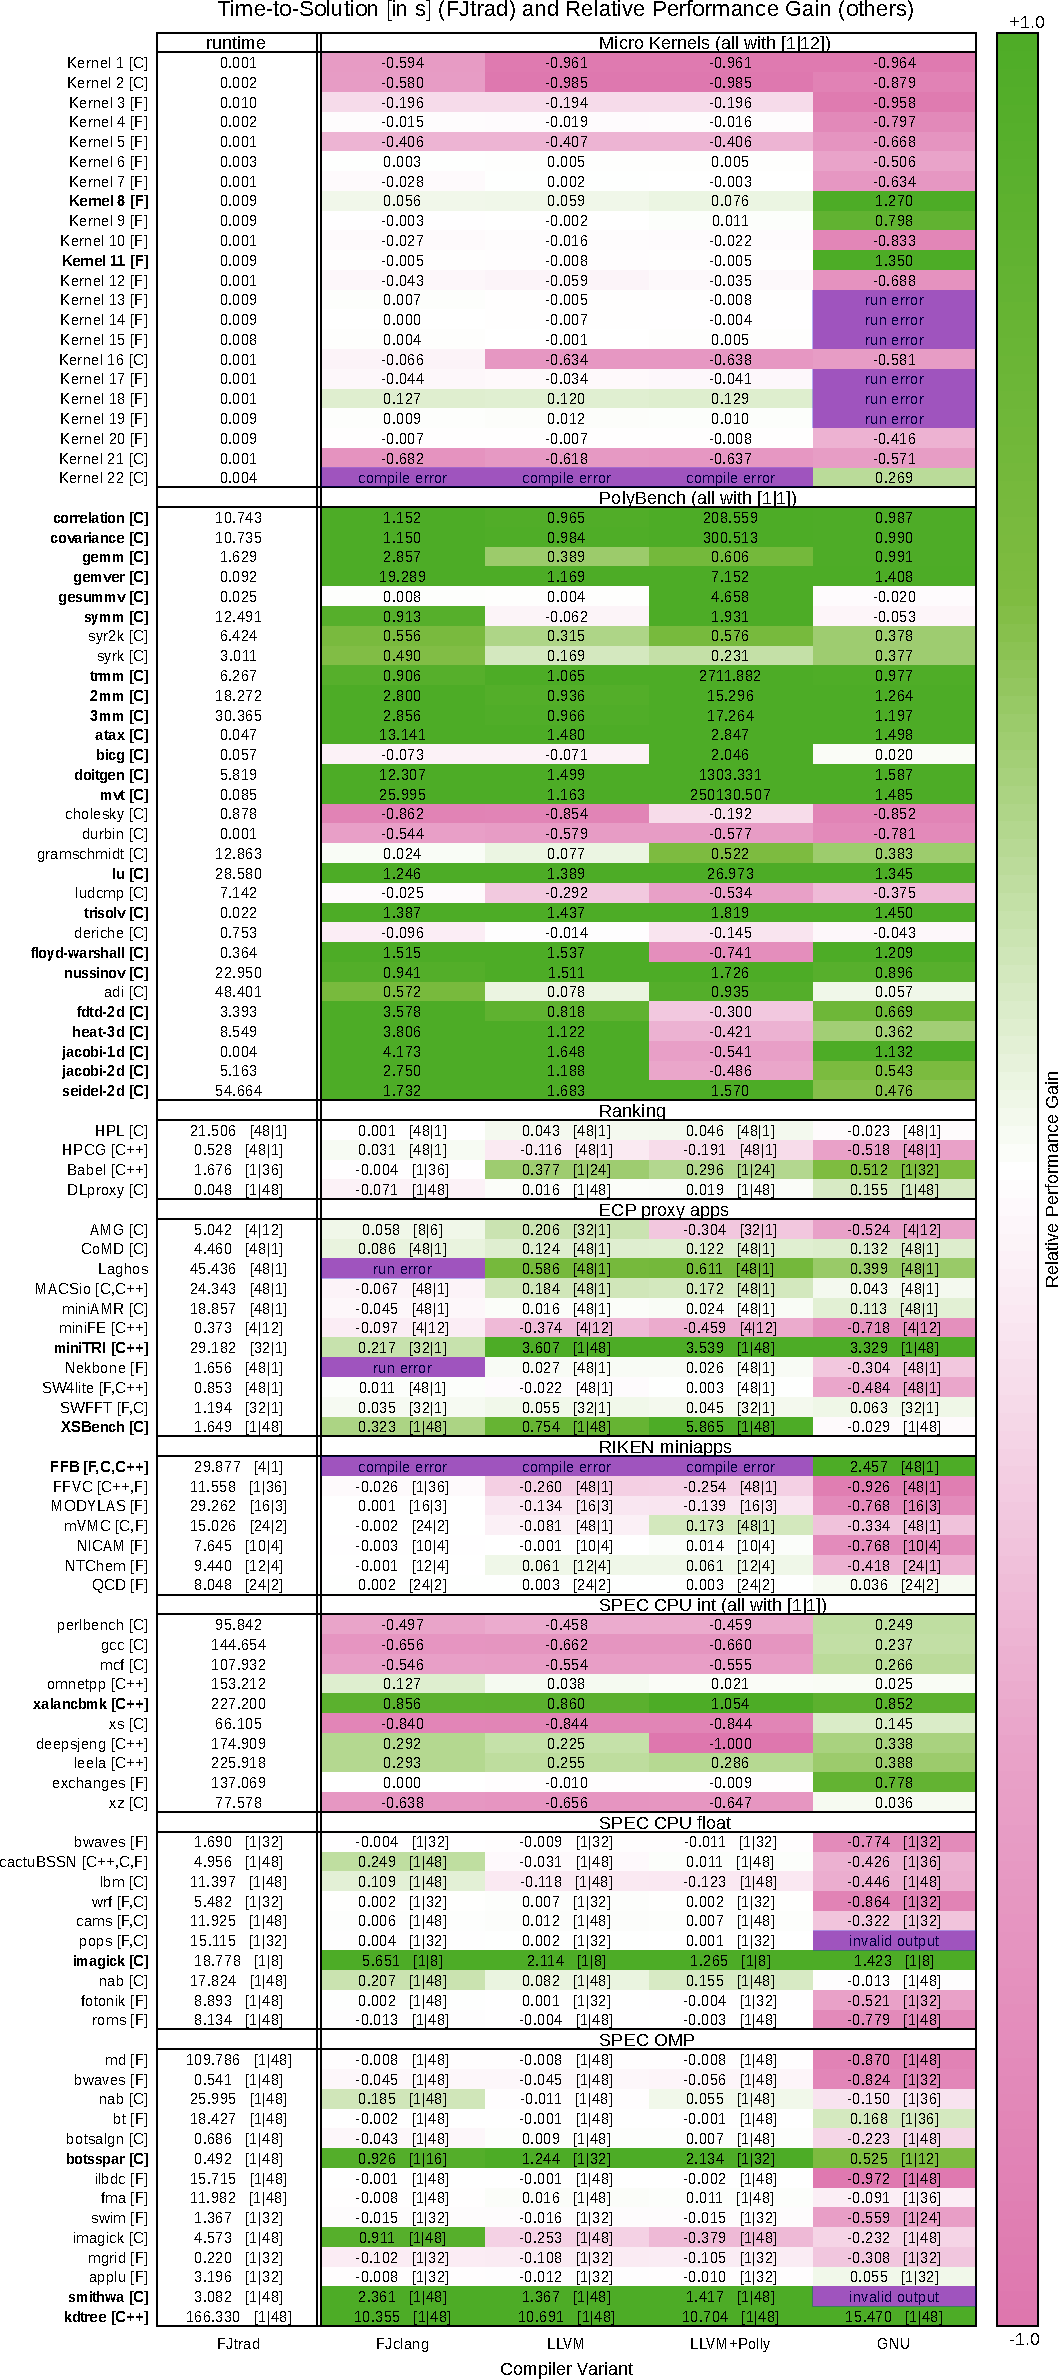
\includegraphics[width=1.085\linewidth]{compiler_compare}
    \caption{Absolute time-to-solution (numbers; \textit{FJtrad} column) and relative gain over \textit{FJtrad} (numbers; color coding; non-\textit{FJtrad} columns)
    for all benchmarks; Invalid entries explain (e.g. ``compiler error'', see Kernel 22); Programming
    language indicated after benchmark name; Benchmark names with $>$2x speedup in bold; Number of MPI rank \& OMP threads in brackets}
    \label{fig:compare_compiler}
%    \vspace{-1.6cm}
\end{figure}

\subsection{Micro Kernels and Polybench}\label{sec:eval:micro}
For the Micro Kernels representing RIKEN's priority apps, we clearly see the results
of the co-design efforts for Fugaku. Fujitsu's compiler in traditional mode outperforms
all other compilers in nearly all test. Only the GNU compiler is able to noticeably beat \textit{FJtrad}
in 4 of the 22 tests, but also produces 6 executables which result in runtime errors.
Assuming that we switch always to the best compiler option, then we could reduce the runtime by 17\% on
average, with a median of 0\%, and peak of 2.4x improvement.
However, for PolyBench the roles reverse, with \textit{LLVM+Polly} showing the best results,
followed by \textit{FJclang} in some cases. Especially for \textit{mvt} the polyhedral optimizations
resulted in over 250.000x speedup. Choosing the best compiler over \textit{FJtrad} results in
a median speedup of 3.8x. It remains to be seen if \textit{polly}'s gains translate to
``real'' scientific codes hereafter.

\subsection{TOP500, ECP, and Fiber Proxys}\label{sec:eval:proxy}
HPL gains a minor advantage ($\approx$5\%) by using LLVM over Fujitsu's compilers, despite that
most of the calculations are performed within SSL2, which holds true for the convolution kernel
of the deep learning proxy, too. BabelStream shows the largest gain from switching to LLVM or GNU
with up to 51\% lower runtime. With a few exceptions, like FFB and mVMC, Fujitsu dominates the
other compilers on Fiber mini-apps, which is consistent with the Micro Kernel results shown earlier.
For ECP proxy-apps the conclusions reverses, and the user would be advised to switch to LLVM or
GNU in almost all cases. Such a change leads to an average speedup of 1.65x (median 1.09x).
The 6.7x speedup for XSBench is salient, because it also demonstrates that \textit{polly}
can have an impact on real workloads.

\subsection{SPEC CPU and OMP}\label{sec:eval:spec}
The SPEC measurements reveal multiple interesting insights. Firstly, \textit{FJtrad} outperforms
any Clang-based alternative on A64FX on integer-intensive codes; however, the GNU compiler almost
universally beats \textit{FJtrad} at the same single-threaded workloads. We speculate that this
advantage is partially a result of GNU's prevalence in the embedded space where many of the Arm CPUs have no floating-point
units, and also a result of Arm's continued investments into the open-source GNU compilers~\cite{christina_blog_2020}.
By contrast, for multi-threaded and floating-point-based SPEC CPU workloads, as well as SPEC OMP,
the GNU compiler is currently the worst choice on A64FX. Furthermore, many of the applications
are written in Fortran, and hence there is little benefit (apart from maybe link-time-optimizations)
for switching to LLVM. For C/C++ applications on the other hand, LLVM-based compilers (incl.~\textit{FJclang}),
and \textit{GNU} in a few cases, can yield a runtime benefit over \textit{FJtrad}. We see speedup as high as
16.5x in SPEC OMP simply by switching compilers (e.g., for kdtree), with an average improvement of 49\% in SPEC
CPU and 2.5x speedup in SPEC OMP. The median runtime improvement from choosing the best compiler across
both SPEC suites is 14\%.

Overall, across all 108 benchmarks and realistic workloads, we see that a median runtime improvement of 16\% is possible by
selecting an appropriate compiler, without any changes to the source code or other tuning methods.


\section{Related Work}\label{sec:relwork}
Various publications and reports of A64FX evaluations have been released recently. For
example,~\cite{huber_case_2021} tested LLVM and its SVE code generation capabilities for DCA++,
and~\cite{burford_ookami_2021} compared a limited set of applications with LLVM, GNU, ARM, and Cray
compilers and focused on SVE and multi-node scaling. Similarly,~\cite{michalowicz_comparing_2021}
investigated OpenMP-scaling of 3 proxy apps on A64FX while comparing 5 compilers,
and~\cite{poenaru_evaluation_2021} measured nearly a dozen proxy apps (different from ours) on ARM
and x86 for multiple compilers, but lacked LLVM. In~\cite{alappat_performance_2020}, the authors analyzed
the achievable bandwidth for a set of memory-bandwidth-bound kernels using GNU, and~\cite{sreepathi_e3sm_2021}
reported a 2x performance advantage of GNU compilers for the E3SM climate code. 
Lastly, the studies~\cite{jackson_investigating_2020,odajima_preliminary_2020,sato_co-design_2020}
compare A64FX with Fujitsu's traditional mode to ARM-based ThunderX2 and Intel Xeon CPUs using
various priority apps and proxies.
All these studies are complementary to our comprehensive compiler comparison for a wide
variety of workloads, since they use different apps, compilers, or evaluation approaches.

%XXX \cite{huber_case_2021}
%https://arxiv.org/pdf/2106.14332.pdf tested llvm and its SVE code generation capabilities for  DCA++ but didnt comapre to other compilers
%XXX \cite{burford_ookami_2021}
%https://arxiv.org/pdf/2106.08987.pdf compared a limited set of applications with llvm, gcc, arm, cray
%compilers on aircooled a64fx with focus on sve and multi-node scaling, which complements our study
%XXX \cite{alappat_performance_2020}
%https://arxiv.org/pdf/2009.13903.pdf analyzed the achievable bandwdith for a set of microkernels on aircooled a64fx using gcc
%XXX \cite{jackson_investigating_2020}
%https://arxiv.org/pdf/2009.11806.pdf tested a64fx against thunderrx2 and xeon nodes on a handful of applications, but only using FJtrad, however we used their tuned nekbone flags in our study
%XXX \cite{poenaru_evaluation_2021}
%An Evaluation of the Fujitsu A64FX for HPC Applications measured nearly a dosent proxy applications
%using arm and x86based systems and various compilers, but lacks llvm, highly complementary to our study since the proxy app selection does not overlap
%XXX \cite{odajima_preliminary_2020}
%Preliminary Performance Evaluation of the Fujitsu A64FX Using HPC Applications comparisons of FJtrad to arm on thunderx and intel on xeon
%XXX \cite{sato_co-design_2020}
%https://dl.acm.org/doi/pdf/10.5555/3433701.3433763 testing various priority apps against tx2 and xeon but onl fjtrad on aircooled (also use for fugaku ref)
%XXX \cite{sreepathi_e3sm_2021}
%https://e3sm.org/e3sm-pathfinding-on-fugaku/ concluded that gnu was twice as fast as fj compiler on kernels of the E3SM climate modelling code
%XXX \cite{michalowicz_comparing_2021}
%https://arxiv.org/pdf/2106.09787.pdf investigated omp scaling of 3 proxy apps on a64fx comparing 5 compilers, complementing our study

% An example of a floating figure using the graphicx package.
% Note that \label must occur AFTER (or within) \caption.
% For figures, \caption should occur after the \includegraphics.
% Note that IEEEtran v1.7 and later has special internal code that
% is designed to preserve the operation of \label within \caption
% even when the captionsoff option is in effect. However, because
% of issues like this, it may be the safest practice to put all your
% \label just after \caption rather than within \caption{}.
%
% Reminder: the "draftcls" or "draftclsnofoot", not "draft", class
% option should be used if it is desired that the figures are to be
% displayed while in draft mode.
%
%\begin{figure}[!t]
%\centering
%\includegraphics[width=2.5in]{myfigure}
% where an .eps filename suffix will be assumed under latex, 
% and a .pdf suffix will be assumed for pdflatex; or what has been declared
% via \DeclareGraphicsExtensions.
%\caption{Simulation results for the network.}
%\label{fig_sim}
%\end{figure}

% Note that the IEEE typically puts floats only at the top, even when this
% results in a large percentage of a column being occupied by floats.


% An example of a double column floating figure using two subfigures.
% (The subfig.sty package must be loaded for this to work.)
% The subfigure \label commands are set within each subfloat command,
% and the \label for the overall figure must come after \caption.
% \hfil is used as a separator to get equal spacing.
% Watch out that the combined width of all the subfigures on a 
% line do not exceed the text width or a line break will occur.
%
%\begin{figure*}[!t]
%\centering
%\subfloat[Case I]{\includegraphics[width=2.5in]{box}%
%\label{fig_first_case}}
%\hfil
%\subfloat[Case II]{\includegraphics[width=2.5in]{box}%
%\label{fig_second_case}}
%\caption{Simulation results for the network.}
%\label{fig_sim}
%\end{figure*}
%
% Note that often IEEE papers with subfigures do not employ subfigure
% captions (using the optional argument to \subfloat[]), but instead will
% reference/describe all of them (a), (b), etc., within the main caption.
% Be aware that for subfig.sty to generate the (a), (b), etc., subfigure
% labels, the optional argument to \subfloat must be present. If a
% subcaption is not desired, just leave its contents blank,
% e.g., \subfloat[].


% An example of a floating table. Note that, for IEEE style tables, the
% \caption command should come BEFORE the table and, given that table
% captions serve much like titles, are usually capitalized except for words
% such as a, an, and, as, at, but, by, for, in, nor, of, on, or, the, to
% and up, which are usually not capitalized unless they are the first or
% last word of the caption. Table text will default to \footnotesize as
% the IEEE normally uses this smaller font for tables.
% The \label must come after \caption as always.
%
%\begin{table}[!t]
%% increase table row spacing, adjust to taste
%\renewcommand{\arraystretch}{1.3}
% if using array.sty, it might be a good idea to tweak the value of
% \extrarowheight as needed to properly center the text within the cells
%\caption{An Example of a Table}
%\label{table_example}
%\centering
%% Some packages, such as MDW tools, offer better commands for making tables
%% than the plain LaTeX2e tabular which is used here.
%\begin{tabular}{|c||c|}
%\hline
%One & Two\\
%\hline
%Three & Four\\
%\hline
%\end{tabular}
%\end{table}


% Note that the IEEE does not put floats in the very first column
% - or typically anywhere on the first page for that matter. Also,
% in-text middle ("here") positioning is typically not used, but it
% is allowed and encouraged for Computer Society conferences (but
% not Computer Society journals). Most IEEE journals/conferences use
% top floats exclusively. 
% Note that, LaTeX2e, unlike IEEE journals/conferences, places
% footnotes above bottom floats. This can be corrected via the
% \fnbelowfloat command of the stfloats package.




\section{Conclusion}\label{sec:concl}
In conclusion, we demonstrate a clear benefit from exploring alternative compilers for the A64FX CPU as a valid first-order
tuning method before investing a considerable amount of effort into testing ``exotic'' compiler flags, environment variables, and
performing manual code refactoring.
Especially, the performance discrepancy for PolyBench, which we show in Figure~\ref{fig:demo_polly}, was
solved by switching from the recommended \textit{FJtrad} to LLVM 12 compiler, but the \textit{polly}
optimizations seem rarely applicable or beneficial outside this benchmark set.
To revisit our initial question,
we could not identify a ``silver bullet'' compiler for A64FX, but our measurements give indications
for which compilers work well in which situations, i.e., Fujitsu for Fortran codes, GNU for integer-intensive
apps, and any clang-based compilers for C/C++. Furthermore, we noticed that for ``legacy'' applications, the
recommended usage model of 4 ranks and 12 threads per A64FX node results in suboptimal time-to-solution
more often than not, and that the Arm software ecosystem for HPC is not as mature as for x86, yet.

Our work is just one among many similar, early explorations of the newly introduced Arm-base CPU
for high-performance computing, but it gives reason to believe that potential performance deficiencies, when
directly compared against x86 for the same applications, are most likely the results of immature compilers.
Hence, our recommendation to administrators and users of A64FX-based supercomputers is to install and test as
many different, available compilers as possible to extract the true performance potential from the
A64FX CPU. Similarly, it could be worthwhile to revisit how various system libraries, such as for searching, sorting, routing,
or MPI libraries, etc., and other OS packages are (pre-)compiled for the A64FX processor.

%- polly rarely translates to real codes
%- no silver bulltet, but FJ best for fortran, gnu best for integer-intensive codes, clang-based compilers best
%for c/c++ 
%- implication for system software, such as sorting, routing, mpi libs and late3ncy, to name a few, since they are 
%currently precompiled (OS stuff) or compiled with FJ's tools
%- user need to investigate their codes and compiler options since there is no mature, go-to compiler yet
%- admins should make as many compilers available as possible and document the benefits of exploring the options
%	\item Is the recommended usage model for A64FX, i.e., compiler+flags as well as number of MPI/OMP ranks
%	and threads, ideal or just a starting point?
%	\item Is there a ``silver bullet'' compiler choice for A64FX?
%	\item Can performance differences, compared to similar x86-based hardware, be attributed to the compiler?

% conference papers do not normally have an appendix


% use section* for acknowledgment
\ifCLASSOPTIONcompsoc
  % The Computer Society usually uses the plural form
  \section*{Acknowledgments}
\else
  % regular IEEE prefers the singular form
  \section*{Acknowledgment}
\fi

The authors would like to thank various colleagues from RIKEN R-CCS, in particular members of the NG-HPA, HPAI, and 
Operations team, for their feedback, discussions, and assistance with software installation and application debugging.
This work was supported by the Japan Society for the Promotion of Science KAKENHI Grant Number JP19H04119;
and by the New Energy and Industrial Technology Development Organization (NEDO).



% trigger a \newpage just before the given reference
% number - used to balance the columns on the last page
% adjust value as needed - may need to be readjusted if
% the document is modified later
%\IEEEtriggeratref{8}
% The "triggered" command can be changed if desired:
%\IEEEtriggercmd{\enlargethispage{-5in}}

% references section

\bibliographystyle{IEEEtran}
\bibliography{IEEEabrv,a64fxCvC}

% can use a bibliography generated by BibTeX as a .bbl file
% BibTeX documentation can be easily obtained at:
% http://mirror.ctan.org/biblio/bibtex/contrib/doc/
% The IEEEtran BibTeX style support page is at:
% http://www.michaelshell.org/tex/ieeetran/bibtex/
%\bibliographystyle{IEEEtran}
% argument is your BibTeX string definitions and bibliography database(s)
%\bibliography{IEEEabrv,../bib/paper}
%
% <OR> manually copy in the resultant .bbl file
% set second argument of \begin to the number of references
% (used to reserve space for the reference number labels box)
%\begin{thebibliography}{1}
%
%\bibitem{IEEEhowto:kopka}
%H.~Kopka and P.~W. Daly, \emph{A Guide to \LaTeX}, 3rd~ed.\hskip 1em plus
%  0.5em minus 0.4em\relax Harlow, England: Addison-Wesley, 1999.
%
%\end{thebibliography}




% that's all folks
\end{document}


